\chapter{IEEE 802.11}

\begin{figure}[htbp]
   \centering
   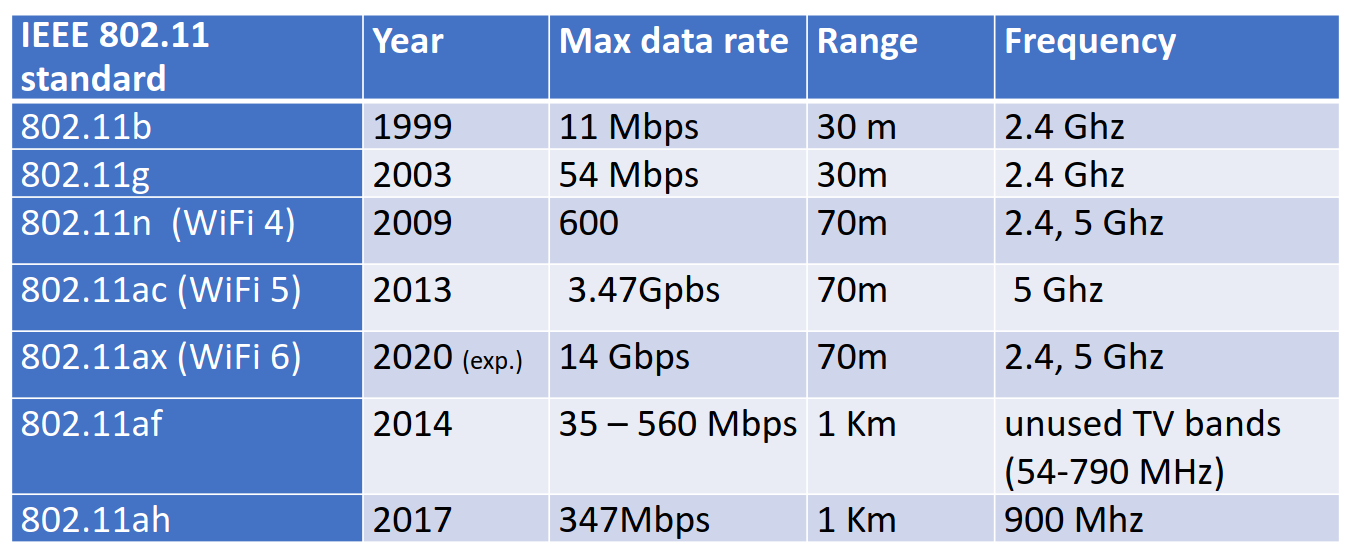
\includegraphics{images/ieee_bgn.png}
   \caption{IEEE 802.11 standards}
   \label{fig:ieee_bgn}
   All these standards \texttt{use \texttt{CSMA/CA} for multiple access}, and have base-station and ad-hoc network versions
\end{figure}

IEEE 802.11 standards refer to the \textit{Physical} Layer.
In case of an AP (Access Point), every station must channel its communication through the AP to talk to any other. Otherwise, in an \textit{Ad-Hoc} network, stations can communicate directly with each other.

TODO

\note{TODO non ci sono domande su questa cose nel pdf}